\documentclass[11pt, oneside]{article}   	% use "amsart" instead of "article" for AMSLaTeX format
\usepackage{geometry}                		% See geometry.pdf to learn the layout options. There are lots.
\geometry{letterpaper}                   		% ... or a4paper or a5paper or ... 
%\geometry{landscape}                		% Activate for rotated page geometry
\usepackage[parfill]{parskip}    		% Activate to begin paragraphs with an empty line rather than an indent
\usepackage{graphicx}				% Use pdf, png, jpg, or eps§ with pdflatex; use eps in DVI mode
								% TeX will automatically convert eps --> pdf in pdflatex		
\usepackage{amssymb}
\usepackage{color}
\usepackage{subcaption}
\usepackage{caption}

\newcommand{\todo}[1]{ \textcolor{red}{\bf{To Do:} #1}}
\newcommand{\toref}[1]{ \textcolor{blue}{\bf{REFERENCE #1}}}
\newcommand{\future}[1]{ \textcolor{green}{\bf{Future Direction: #1}}}

%SetFonts

%SetFonts


\title{6 Month TAP Report}
\author{By Me :)}
\date{}							% Activate to display a given date or no date

\begin{document}
\maketitle

\section{Wounds and Plasma Treatment}
Plasmas are rapidly extending into the field of medicine, with potential application in wound healing \cite{Haertel2014nonthermal, Isbary2013nonthermal}, cancer treatment \cite{Hirst2016low, Fridman2007floating}, coagulation \cite{Fridman2006blood, Chen2009blood} and sterilisation \cite{Fridman2006blood, Laroussi2002nonthermal}.
Applications such as these pertain to plasmas ability to interact with living biological substrates such as bacteria, both in planktonic and biofilm forms \cite{Joshi2010control, Pei2012inactivation, Ziuzina2015cold} and eukaryotic, mammalian cells \cite{Haertel2014nonthermal}.
For sterilisation applications, the properties of low temperature plasma, in particular the low temperature and ability to operate at atmospheric pressure, allow their use both on equipment surfaces \cite{Laroussi2002nonthermal} and also directly on biological tissue, for example chronically infected wounds \cite{Haertel2014nonthermal, Isbary2013nonthermal, Fridman2006blood}.

This project is concerned with wound healing and how low temperature air plasma can be developed to allow treatment of wounds.
Plasmas can be used on wounds with two aims:
\begin{enumerate}
\item Bacterial killing
\item Host cell activation and healing promotion
\end{enumerate}

While exact mechanisms of action are not fully understood, there have been investigations into the roles of the different plasma components.
Briefly, low temperature plasmas are very weakly ionised gases (degree of ionisation $<$ 1\%), with a global temperature of of approximately room temperature ($< 40^{\circ} C$), and dry reactive environment, allowing direct contact with biological substrates.
Electrons liberated in the plasma mediate the different plasma components, for example, dissociation of molecules, yielding reactive radical species, emission as a result of electron impact electronic excitation and ionisation which yields ions and allows plasma sustainment.
It is, therefore, likely that the efficacy seen so far using plasmas is due to this complex plasma composition, and also what suggests that bacteria are going to be less likely to build up resistance, due to the multimodal nature of the plasma treatment.

The main three components that will be discussed in the next sections are charged particles and associated electric fields, emission of, for example UV photons, and reactive neutral species.


\subsection{Bacterial Killing}
\subsubsection{RONS}
LTP is a highly efficient source of reactive species, produced by mechanisms such as electron impact excitation and dissociation.
The gas present in the plasma determines the types of species that will be produced. 
In the case of air plasma, reactive oxygen and nitrogen species (RONS) are readily produced and these have multiple possible effects on biological substrates.
Important species produced include atomic oxygen (O), ozone (O$_3$), singlet delta oxygen (O$_2$($^1\Delta$)), superoxide (O$_2^-\cdot$), atomic nitrogen (N), hydroxyl radicals (OH), hydrogen peroxide (H$_2$O$_2$) and various nitrogen oxides (NO, NO$_2$ and N$_2$O) \cite{Graves2014low}.

Whilst reactive species were thought to be purely damaging molecules produced in the body which only serve to promote disease and ageing \cite{Harman1955aging}, it is now known that their role is far more complex than this, and that reactive species have crucial roles to play in the immune system and in normal physiological signalling \cite{Thannickal2000reactive}.
At low concentrations, RONS are vital to human health. 
For example, they are important cell signalling regulating molecules in cells such as fibroblasts, endothelial cells and smooth muscle cells.
Further to this, they are essential for host defence as they are produced by immune cells during an immune response in order to kill invading pathogens.
The importance of this function is shown by patients with chronic granulomatous disease (CGD), who cannot synthesise the superoxide radical (O$_2^-\cdot$) resulting in multiple, persistent infections \cite{PhamHuy2008free, Fang2004antimicrobial}.


If the concentrations of RONS become excessive and there is an imbalance between radical formation and neutralisation, then they can become dangerous, causing damage to lipids, proteins and DNA \cite{PhamHuy2008free}.
Considering plasma treatments containing ROS, these exogenous species can enter the cells, or induce the formation of new ROS intracellularly and exert their action \cite{Haertel2014nonthermal}.
RONS can be visualised inside cells using fluorescent dyes, an example of which is shown by the likes of Joshi \textit{et al} \cite{Joshi2010control}.

Oxidative attack on lipids inside cells or as part of cell membranes results in a chain reaction and the formation of harmful products, the most mutagenic and toxic being malondialdehyde (MDA) and 4-hydroxynonenal (4-HNE), respectively \cite{Ayala2014lipid}.
Lipid peroxidation occurs as a chain reaction, mediated by free radicals, with the hydroxyl radical ($\cdot$OH) being particularly effective.
Firstly, the radical breaks an unsaturated carbon bond in the lipid, abstracts a hydrogen and forms a lipid radical, which then readily reacts with oxygen to form a lipid peroxy radical.
The lipid peroxy radical can then attack another lipid and abstract a hydrogen, forming a new lipid radical and a lipid hydroperoxide. 
Thus the process propagates until antioxidants such as vitamin E can neutralise the radical species \cite{Ayala2014lipid}.

Proteins can be changed structurally and enzymes break \cite{PhamHuy2008free}.

As with lipid peroxidation, the $\cdot$OH radical is effective for damaging DNA. 
There are many ways it can interact with the components of DNA, in particular through reactions with the purines and pyrimidines of DNA.
Although the body has many DNA repair mechanisms in place, mutations as a result of the oxidative insult still occur.
These are often result in mispairing of DNA bases and subsequent transversion mutations.
For example, a common lesion formed in DNA is 8-OH-Gua (a guanine base that has been modified through attack by $\cdot$OH), which wrongly pairs with adenine and thus results in a G $\rightarrow$ T transversion mutation \cite{Dizdaroglu2012oxidatively}.
It readily reacts with nucleotide bases, which allows for frequent mutations 
DNA attack can cause mutations. \cite{PhamHuy2008free}.






\subsubsection{UV}
UV emission is known to be harmful at certain wavelengths and powers, and, as such, it has been used extensively for sterilisation purposes due to it's ability to interfere with DNA \cite{Laroussi2004evaluation}.
To investigate the effects of UV radiation emitted from plasmas, windows can be put between the plasma and the sample that allow specific wavelengths of UV radiation through, while blocking all other plasma components. 
Using these methods, there is evidence to suggest that the effects of UV radiation are negligable \cite{Laroussi2004evaluation, Dobrynin2009physical}.
There is currently a lack of safety guidelines relating to the safe dose of UV that can be applied to skin.
Whilst there are suggestions for undamaged skin, there is nothing for broken, damaged skin, therefore, keeping the UV emission as low as possible is probably advisable \cite{Isbary2013cold}.

\subsubsection{Charged Particles and Electric Fields}
As charged particles are generally confined within the strong electric fields within the plasma, they don't tend to travel far outside the plasma bulk.
This means that one method for delineating the roles of electric fields and particles from the other plasma components is by comparing direct (where the biological substrate is in direct contact with the plasma) and indirect (where the biological substrate is only exposed to the plasma effluent) plasma treatments.
Investigations such as this have suggested that charged particles or electric fields, or a combination of both, are important for bacterial killing as direct treatment is much more efficient that indirect treatment \cite{Fridman2007comparison}.
A proposed mechanism for this increased efficacy when charged particles are in contact with the biological sample came from Mendis $et al$ in 2000 \cite{Mendis2000a} who suggested that accumulation of ions on the membranes of cells could cause an electrostatic force greater than the tensile strength of the membrane causing rupture.
This was noted following the observations of Laroussi \textit{et al} \cite{Laroussi1999images} that showed morphological changes and lysis of the treated bacteria.
\todo{Look into electroporation mechanism. Is this just electroporation by plasmas???}

\subsection{Host Cell Activation and Healing Promotion}
It seems that the molecular interactions of plasmas are less well understood when considering the beneficial effects it has on host cells and tissues.
However, by considering the normal, physiological effects of plasma components that are produced endogenously, and the observed outcomes from wound treatment with LTP, mechanisms of action can be proposed.

It is generally accepted that low doses plasma treatment is good for stimulating effects - in the context of wound healing this would include things like increased proliferation and migration and DNA repair. 
This contrasts with higher doses which generally induce damaging/lethal effects such as cell death and DNA damage \cite{Haertel2014nonthermal}. 

There is evidence to show that plasma treatment could accelerate wound healing, both from laboratory experiments, and clinical trials.
For example, following scratch tests, 3T3 keratinocytes treated with plasma recovered and re-grew to confluence more quickly than untreated controls \cite{Tipa2011plasma}.
This suggests that plasma treatment can increase keratinocyte proliferation, something which has also been shown by changes in gene expression in HaCaT keratinocytes following plasma treatment \cite{Barton2013nonthermal}.
Clinically, devices such as KinPen and MicroPlaSter have shown promise when used on human patients, aiding healing without any obvious side-effects \cite{Isbary2013cold, Isbary2012successful, Isbary2010a, Bekeschus2016the}.


%Plasma seems to be toxic to lymphocytes but not neutrophils or monocytes due to strong oxidation in the cell membrane and cytosol. This may be beneficial as excessive lymphocytes are present in pathological wounds and, therefore, by removing them, it may promote healing \cite{Bekeschus2016the}.
%\toref{Kramer2013suitability, Haertel2014, Bender2012, Brehmer2015, Joshi, Kong2009}
Dealing with the groups of plasma components, there is proposed mechanisms of action for RONS and electric fields in wound healing.
However, the actions of RONS and electric fields discussed below is not determined using plasma treatment, therefore, it can only be proposed that the same actions are carried out by plasma-produced species rather than endogenously produced species.


\subsubsection{RONS}
There is much evidence showing the importance of RONS in the normal, physiological process of wound healing.
Throughout the different stages of healing, RONS have a role to play.
Firstly, RONS are important for coagulation through involvement in the release of tissue factor (TF), which triggers the clotting cascade. RONS are also important for platelet recruitment and activation, subsequent further release of ROS and more TF production \cite{Soneja2005role}.
It is possible that plasma derived RONS can also carry out this function, as shown by multiple studies of plasma on coagulation \cite{Fridman2006blood, Chen2009blood}.

RONS are also important for the inflammatory, re-epithelialisation and wound contraction stages of wound healing.
This is particularly due to their ability to act as signalling molecules and also their role in mediating the release of factors and receptor affinity.
These roles help control chemotaxis and adhesion of immune cells recruited to the wound site and help the activation and proliferation of keratinocytes to start re-epithelialisation of the wound \cite{Soneja2005role}.
RONS are also involved in collagen production and control of myofibroblast (the cells which contract to decrease the wound area) formation \cite{Soneja2005role}.


Nitric oxide (NO) is a very important species in wound healing and contributes to all the processes above.
The potential for using NO therapeutically for wound healing applications has been investigated.
For example Shekhter \textit{et al} \cite{Shekhter2005beneficial} used an air plasma device, named 'plason', to produce an NO-containing gas flow which was then used to treat wounds in rats. 
The NO was produced by a high temperature electric arc discharge, and then the gas was allowed to cool before being used on the wounds. 
Wounds treated with 'plason' showed accelerated healing compared to the control group.
However, what I find unclear is how they know there was only NO in the gas, surely other species would also be present in the gas?

%Inflammation: Following immune cell recruitment to the wound site, they produce many factors important for potentiating the immune response. Species such as H$_2$O$_2$ are important secondary messenger molecules for these factors and are, therefore, important during an immune response. RONS in general are also important for affecting chemotaxis and adhesion of immune cells such as neutrophils and monocytes \cite{Soneja2005role}.
%
%Re-epithelialisation: ROS are important for promoting collagenase expression (for wound remodelling) and epidermal growth factor (EGF) expression, which promotes the proliferation of keratinocytes into the wound site \cite{Soneja2005role}.
%
%Angiogenesis: ROS also play a role in promoting angiogenesis, matrix deposition and wound contracture, by enhancing the release of pro-angiogenic factors and enhancing its receptor affinity, stimulating the release of collagen and controlling the transition of fibroblasts to myofibroblasts (the cells which contract to make the wound site smaller) \cite{Soneja2005role}.


\subsubsection{Electric Fields}

Normal plasma membranes have a potential difference across them, due to the movement of ions across the membrane.
When epithelium is broken through wounding, the ion currents are disrupted and an electric field is established.
There is evidence to suggest that this electric field helps guide the migration of epithelial cells during healing \cite{Zhao2009electrical}.
Following this, there have been studies into the effects of using electric fields for the promotion of wound healing \cite{Thakral2013electrical, Messerli2011extracellular}.
However, as with plasma treatment, there is little understanding of the relation between 'dose' and outcomes etc, though looks promising.
Also all the different trials use different regimes and therefore comparison is difficult.
Lab trials show the importance of electrical currents/fields for wound healing, and there are clinical trials involving electric fields for wound healing that show promise \cite{Messerli2011extracellular}.
\todo{E field strengths?? Applied voltages?? Comparison to plasmas}
%The threshold field strength noticeable by cells is 4500 times smaller than that required for electroporation of skeletal muscle \cite{Messerli2011extracellular}.

\section{Work to Date: Plasma Simulations}

For the last few months I have been continuing to work on plasma simulations, using GlobalKin.
As detailed in my previous TAP report, GlobalKin is a 0 dimensional global chemistry plasma model that calculates the time evolution of plasma species, given specific geometry and plasma parameters \cite{Stafford2004O2}.
To do this, it has an internal Boltzmann solver for calculating electron energy distribution functions over time which it then combines with a reaction chemistry module outlining all the species and reactions taking place in the plasma.
Finally, species densities are determined by an ordinary differential equation (ODE) solver to solve ODEs for species densities formed by the reaction chemistry module.
\textbf{Figure \ref{fig:GlobalKin}} is a schematic for how GlobalKin works.
For the chemistry module to work, an input file must be provided which contains all the plasma species and reactions along with a set of parameters.



\begin{figure}
\includegraphics[width=\textwidth]{Figures/GlobalKinDiagram}
\caption{Diagram outlining how GlobalKin works. Firstly, ODEs for species density and electron temperature are constructed. This takes direct GlobalKin inputs specified by the user, as well as electron reaction rate coefficients, diffusion coefficients and mobilities from the Boltzmann solver. An ODE solver then solves the equations and the new species densities are fed back into the ODEs and Boltzmann solver, for new densities to be calculated. At regular intervals, the Boltzmann solver also updates and new coefficients are fed back into the ODEs for the ODE solver to work with. This results in the time evolution of species densities and electron temperatures.}
\label{fig:GlobalKin}
\end{figure}



My project is concerned with the use of air plasmas, therefore, the aim is to develop an air reaction chemistry set for use in GlobalKin.
However, as air is highly complex, involving many species and reactions, I have started with developing a set for pure nitrogen plasmas, which currently includes 31 species and 207 reactions.


\subsection{Nitrogen Chemistry Set}
To begin the chemistry set, Vasco Guerra kindly shared with us his N$_2$:O$_2$ chemistry set used in \cite{Kutasi2016tuning}.
This gives a good starting point for the nitrogen reactions and their rates.

\subsubsection{Species}

The model so far consists of the species outlined in \textbf{table \ref{table:Species}}, in accordance with \cite{Kutasi2016tuning}.
This includes ground state N, N$_2$, N$^+$, N$_2^+$ and N$_4^+$; and various excited states of N$_2$, N$_2^+$ and N.
Being a molecule, nitrogen can absorb energy into its bonds and is said to exist in multiple vibrational states.
For this chemistry set, the first 17 vibrational states of ground state nitrogen are included (N$_2$ (X, v = 0 - 17)).
The N$_2 (a^1\Pi_g/a'^1\Sigma^?_u/w^1\Delta_u)$ states are also included, however, they are currently considered as a single state due to reasons discussed below.



\begin{table}
\caption{Species included in Nitrogen Chemistry Set}
\begin{center}
\begin{tabular}{| c | c |}
\hline
Species & States \\
\hline\hline \hline
N$_2$ & $X^1\Sigma_g^+  (v = 0 - 17),  A^3\Sigma_u^+, B^3\Pi_g, B'^3\Sigma_u^-, C^3\Pi_u, (a^1\Pi_g/a'^1\Sigma^?_u/w^1\Delta_u)$\footnotemark  \\
\hline
N$_2^+$ & $X^2\Sigma_g^+, B^2\Sigma_u^+ $ \\
\hline
N & $^4S, ^2D,  ^2P$ \\
\hline
N$^+$ & - \\
\hline
N$_2^+$ & - \\
\hline
N$_4^+$ & - \\
\hline
\end{tabular}
\end{center}
\label{table:Species}
\caption*{$^1$ These three states are considered as a single state by GlobalKin.}
\end{table}




\subsubsection{Reactions and Rates}

A list of all the possible reactions occurring in the plasma needs to be provided in an input file to GlobalKin.
Each reaction must be listed with it's rate or cross section, which can be found in literature.

\subsubsection*{Electron Reactions}
The rates of electron impact reactions are highly dependent on electron energy, therefore, as electron energies in the plasma change, the rates change accordingly.
To account for this, electron impact cross sections are specified instead of a rate.
The reaction cross section is the probability of a reaction occurring given an electron is at a particular energy.
GlobalKin can then use the cross sections alongside the Boltzmann solver (which calculates the electron energy distribution function at regular intervals) to calculate the reaction rate at particular time points.

GlobalKin contains the electron impact cross sections for most reactions internally and for the time being, only electron impact reactions with cross sections listed in GlobalKin have been included in this chemistry set.
For this reason, the three N$_2$ states of a, a' and w, are all considered as a single state as there is only one cross section listed for all three of these species in GlobalKin.

\subsubsection*{Heavy Particle Reactions}
Heavy particles have a much more constant energy compared to electrons, due to their heavier mass. 
For this reason, reaction rates can be stated as constants, in the Arrhenius equation format.
These rates are found in the literature and the ones being used in the model can be found in the chemistry reaction set attached.


\subsubsection*{Vibrational Kinetics of Nitrogen}

As shown above, nitrogen has many vibrational states, the first 17 of which are included in this chemistry set.
Vibrational states are important to include in nitrogen models due to the fact that these states have an impact on the electron energy distribution function \cite{Guerra2004kinetic}.
This is due to there being a high probability of electrons colliding with N$_2$ molecules and exciting them to different vibrational states (equation \ref{eqn:ElectronVibration}), causing electron energy losses.
\begin{equation}
e^- + N_2(v=0) \rightarrow N_2(v=1) + e^-
\label{eqn:ElectronVibration}
\end{equation}

Also, superelastic collisions of electrons with vibrational states (equation \ref{eqn:SuperelasticVibrational}) cause electrons to gain energy and is a process responsible for high energy electrons \cite{Guerra2004kinetic}. \todo{check!}

\begin{equation}
e^- + N_2(v=1) \rightarrow N_2(v=0) + e^-
\label{eqn:SuperelasticVibrational}
\end{equation}

As well as for their impact on the EEDF, vibrational states can also have an impact on the dissociation of N$_2$, and on gas heating in the plasma \toref{Find a reference}.
For this reason it is important to include the production and destruction mechanisms of vibrational states.
As well as superelastic electron collisions, shown in equation \ref{eqn:SuperelasticVibrational}, vibrationally excited states of nitrogen can also be destroyed by collisions with heavy particles N$_2$ and N, in vibration-translation (V-T), as shown in equations \ref{eqn:V-TN2} and \ref{eqn:V-TN}, respectively.

\begin{equation}
N_2(v=n) + N_2 (v=0) \rightarrow N_2(v=n-1) + N_2(v=0)
\label{eqn:V-TN2}
\end{equation}
\begin{equation}
N_2(v=n) + N \rightarrow N_2(v=n-1) + N
\label{eqn:V-TN}
\end{equation}
As well as V-T reactions, vibrationally excited N$_2$ can also be destroyed through vibration-vibration (V-V) collisions.
The general equation for this is as follows:

\begin{equation}
N_2(v=w) + N_2 (v=n) \rightarrow N_2(v=w-1) + N_2(v=n+1)
\label{eqn:V-V}
\end{equation}

Dissociation of N$_2$ is also influenced by the presence of vibrational states of N$_2$, however, this tends to be at the higher vibrational states (e.g. n = 45), which are not included in this model at the moment. 
The importance of these higher vibrational states will need to be investigated and could be added in at a later date \cite{Guerra2004kinetic}.


\subsubsection{Rates of Reactions Involving Vibrational States}

As with other heavy particle reactions, the rates for these reactions are found in the literature.


The rates for N$_2$-N$_2$ V-T reactions (\textbf{equation \ref{eqn:V-TN2}}) can be found in  \cite{Billing1979vv} for n = 1 - 9 \& 20.
Therefore, it was necessary to fit the data to determine rate coefficients for n = 10 - 17 required for the model.
Exponential, 3rd degree polynomial and linear fits were tested.
These are shown in \textbf{figures \ref{fig:fits}}.
As shown in figures \ref{subfig:Exp} and \ref{subfig:ExpAll}, the exponential fit only worked when n=20 was excluded.

To then check how much difference the fits made to the rates and, therefore, the densities of the vibrational states of N$_2$, the model was run twice, once with rates from the linear fit, and once with rates from the polynomial fit.
From this, vibrational distribution functions (VDFs) were then drawn to see how different they were.
TO draw the VDF, the vibrational state densities are first normalised to the ground state density and then the VDF shows the populations of vibrationally excited N$_2$ compared to the ground state.
Alongside this, the density of atomic nitrogen was also determined to see how this was affected.
The results are shown in \textbf{figure \ref{fig:VDFandN}}.
As shown in the figures, which fit is used makes no difference to either the VDF or the atomic nitrogen density.
In \textbf{figure \ref{subfig:VDF}}, the VDFs for both fits are shown, however, only one line is visible as it is directly on top of the other.
It was, therefore, decided that the linear fit data would be used for the model.



%\begin{table}
%\begin{center}
%\caption{Rates for V-T reactions from \cite{Billing1979vv}}
%\begin{tabular}{| c | c | c | c | c | c | c | c | c | c | c |}
%\hline
%n & 1 & 2 & 3 & 4 & 5 & 6 & 7 & 8 & 9 & 20 \\
%\hline
%Rate ($ \times 10^{-21}$) &0.8 & 1.8 & 3.1 & 5.0 & 7.4 & 11 & 16 & 26 & 38 & 1600 \\
%\hline
%\end{tabular}
%\label{table:BillingRates}
%\end{center}
%\end{table}




\begin{figure}
\begin{subfigure}{0.5\textwidth}
\begin{center}
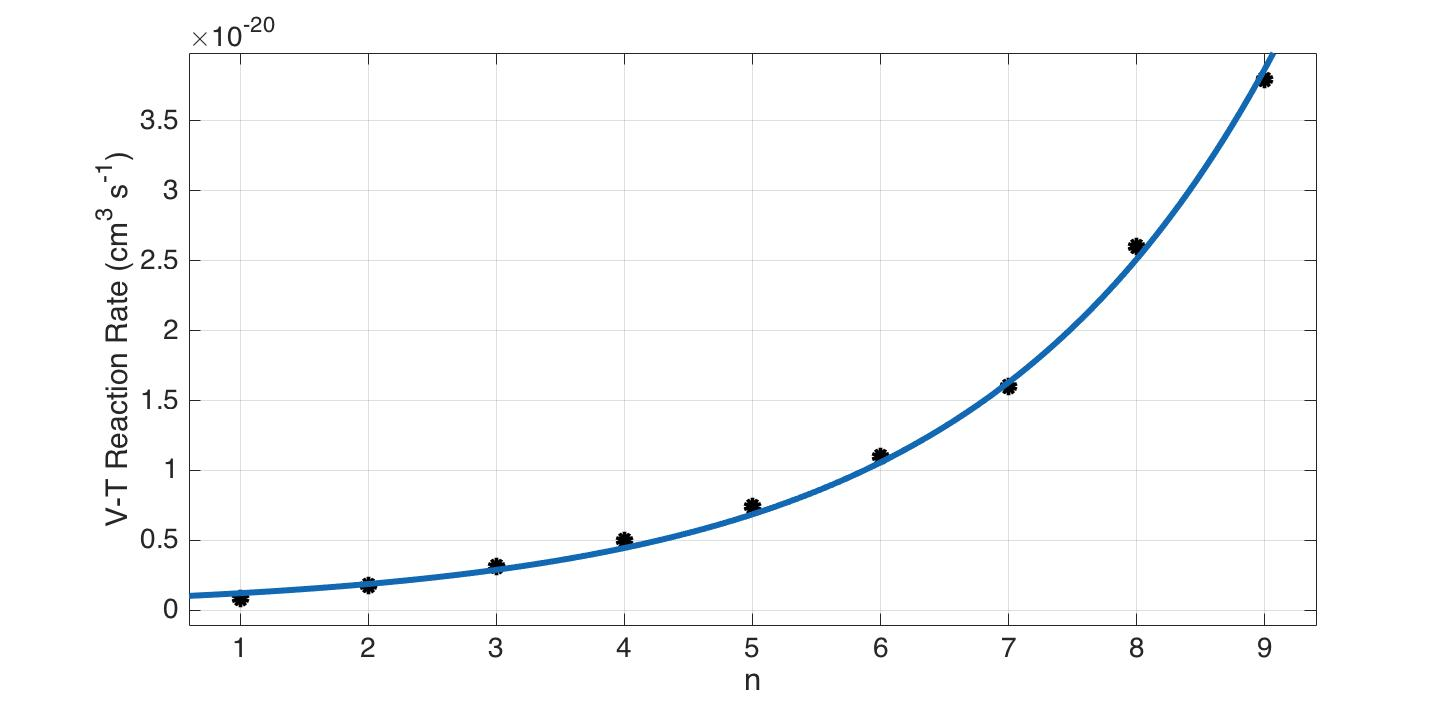
\includegraphics[width=\textwidth]{Figures/ExpFit}
\caption{Exponential Fit for n=1-9}
\label{subfig:Exp}
\end{center}
\end{subfigure}
\begin{subfigure}{0.5\textwidth}
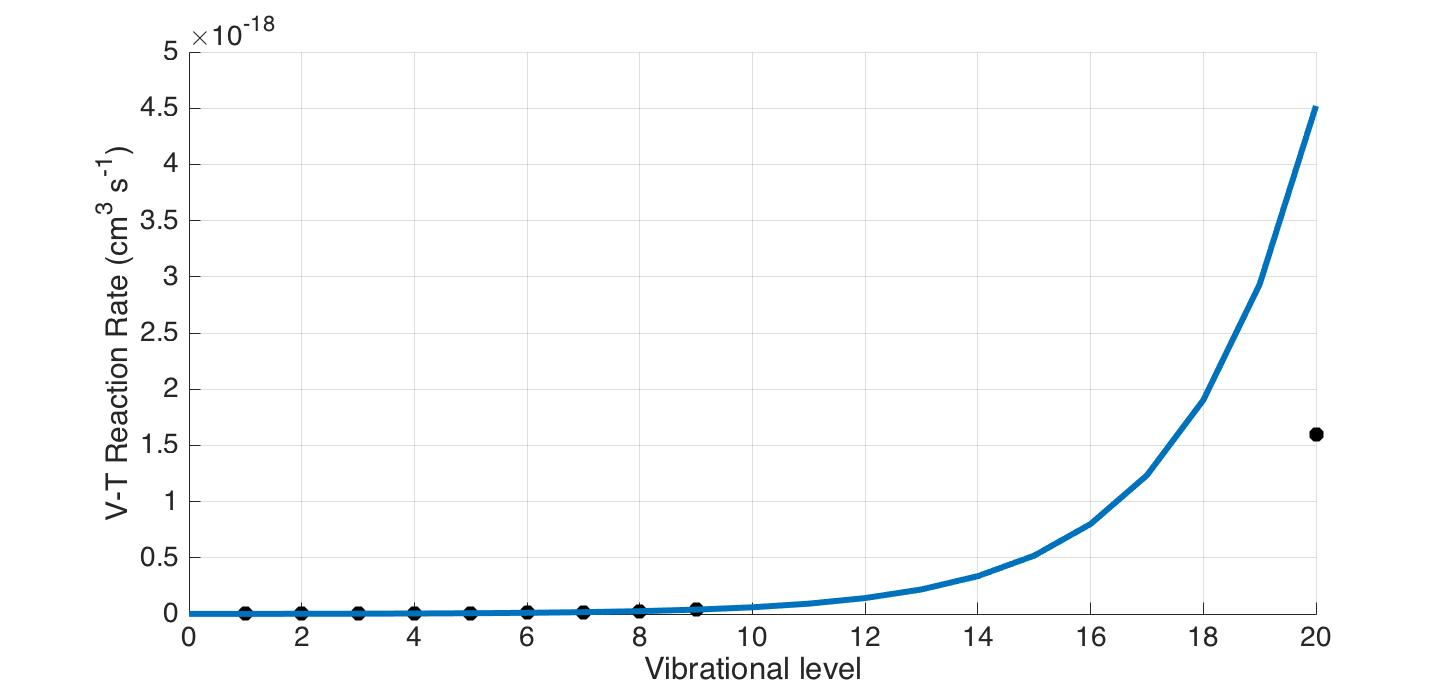
\includegraphics[width=\textwidth]{Figures/ExpFitAll}
\caption{Exponential Fit for n=1-20}
\label{subfig:ExpAll}
\end{subfigure}
\begin{subfigure}{0.5\textwidth}
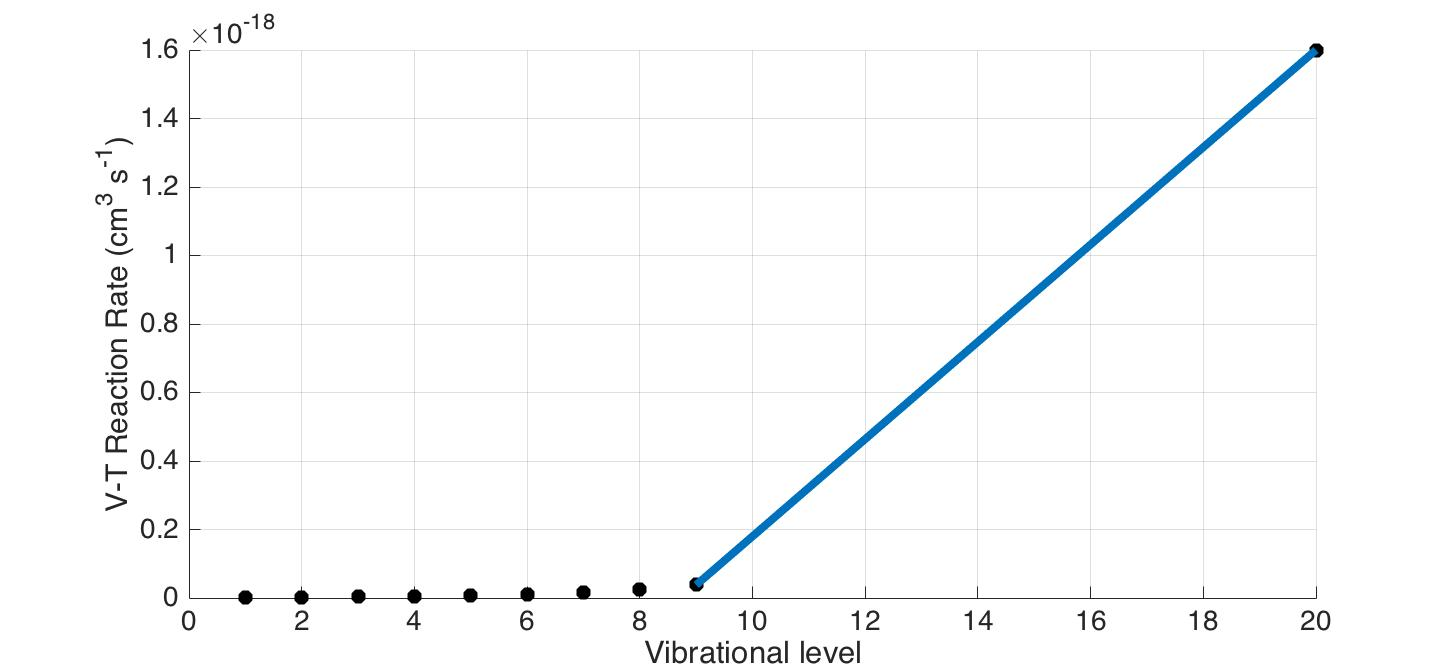
\includegraphics[width=\textwidth]{Figures/Linear}
\caption{Linear fit between n=9 and n=20}
\end{subfigure}
\begin{subfigure}{0.5\textwidth}
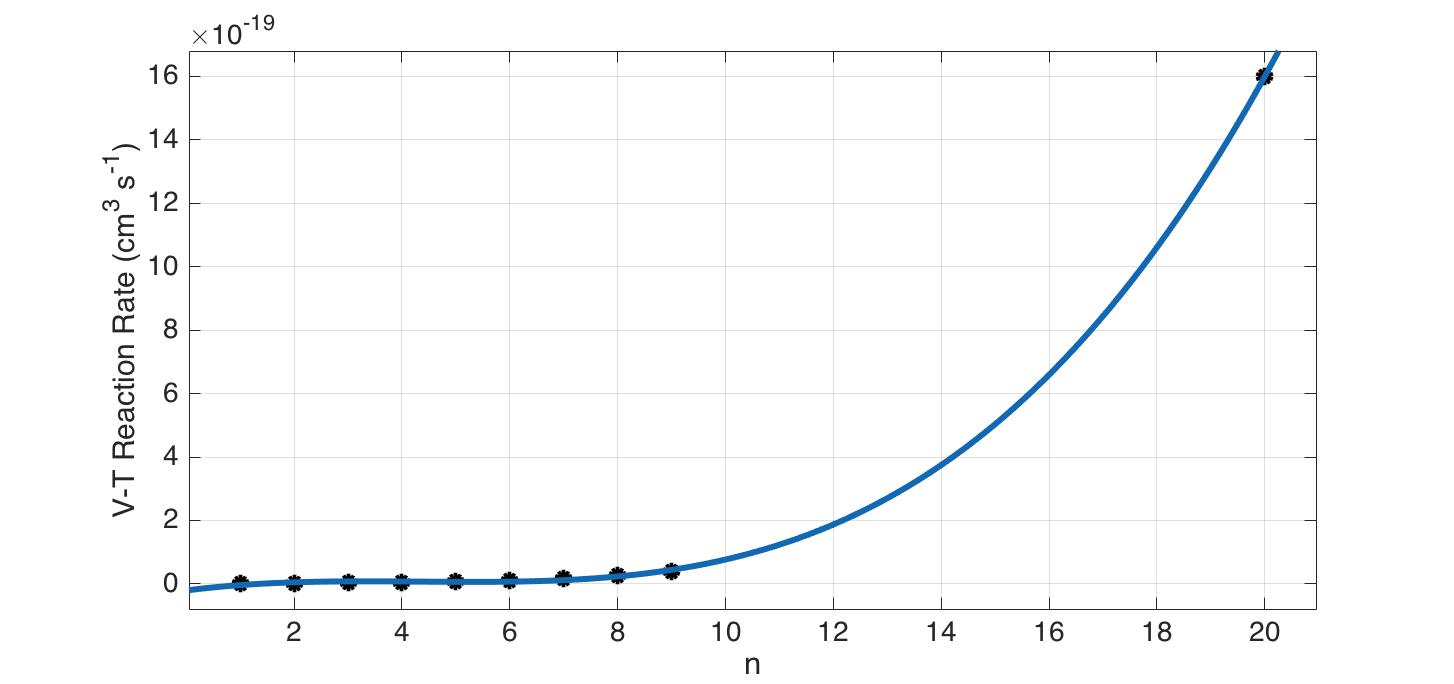
\includegraphics[width=\textwidth]{Figures/Polynomial}
\caption{Polynomial Fit for n=1-20}
\end{subfigure}
\caption{Figure Showing Fitting to V-T reaction rates from Billing and Fisher, 1979 \cite{Billing1979vv}}
\label{fig:fits}
\end{figure}

\begin{figure}
\begin{subfigure}{0.5\textwidth}
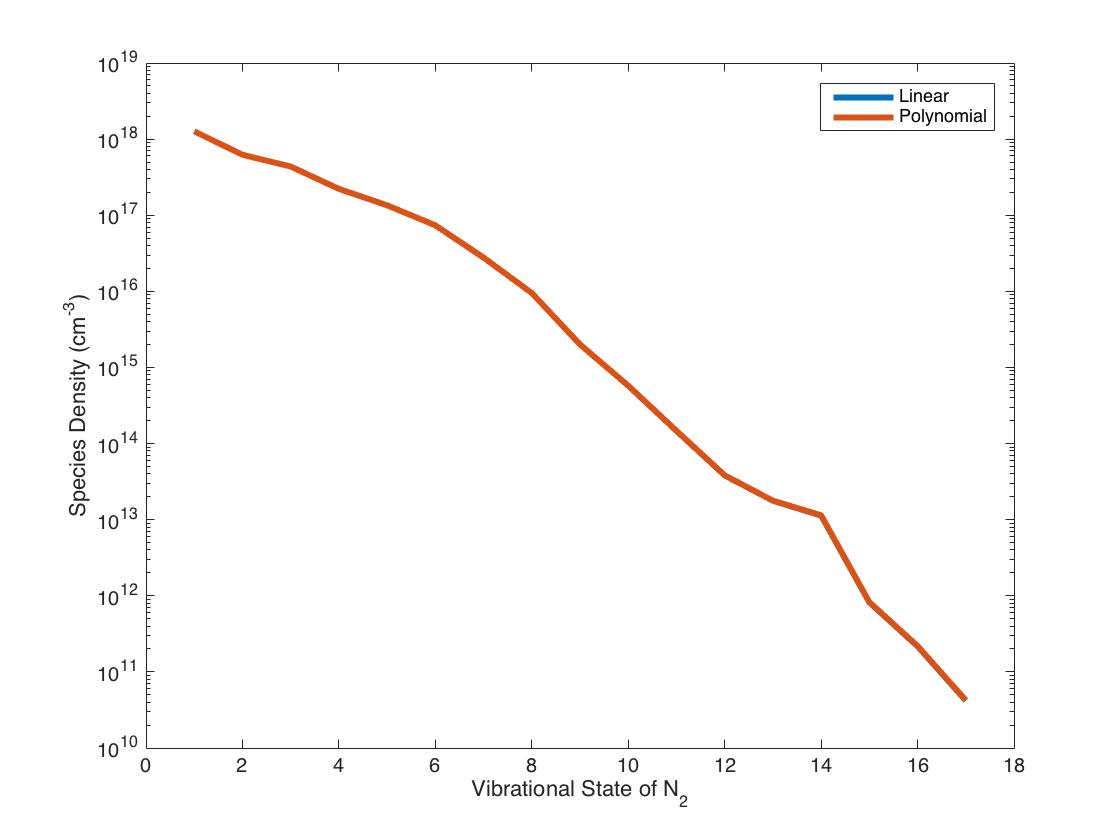
\includegraphics[width=\textwidth]{Figures/VDF}
\caption{Vibrational Distribution Function}
\label{subfig:VDF}
\end{subfigure}
\begin{subfigure}{0.5\textwidth}
\begin{center}
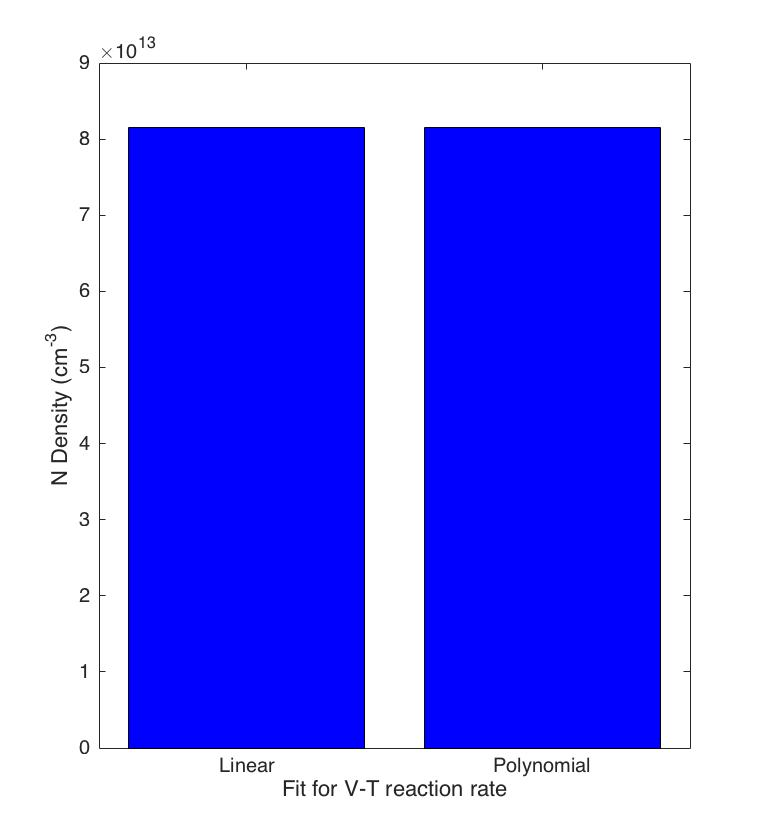
\includegraphics[width=0.7\textwidth]{Figures/Ndensity}
\caption{Atomic Nitrogen Density}
\end{center}
\end{subfigure}
\caption{Graphs showing the vibrational distribution functions and atomic nitrogen densities when different fits are applied to V-T reaction rate data in \cite{Billing1979vv}}
\label{fig:VDFandN}
\end{figure}

Rates for N$_2$-N V-T reactions \textbf{equation \ref{eqn:V-TN}} were taken from \cite{Guerra1995non}.
These rates are being used for the moment, however, Guerra \textit{et al} \cite{Guerra2004kinetic} suggest that they may be too high.
Therefore, it is something to consider changing in time.


Rates for V-V reactions where n = 1 - 9 and n = 20 (\textbf{equation \ref{eqn:V-V}}) were also taken from \cite{Billing1979vv}, with subsequent data fitting.
For these rates, only a linear fit between n = 9 and n = 20 worked, therefore, this is how rates were determined for n = 10 - 17.
Fitting is shown in \textbf{\ref{fig:VVFit}}.

\begin{figure}
\begin{center}
\includegraphics[width=0.7\textwidth]{Figures/VVFitting}
\caption{V-V Reaction Rate Fitting using data from \cite{Billing1979vv}}
\label{fig:VVFit}
\end{center}
\end{figure}

The impact of including these V-V and V-T reactions was then tested by comparing the VDF when both reactions were included compared to only one or the other. 
The rest of the reaction set remained unchanged.
The VDFs are shown in figure \ref{fig:VDFComp}.
From this, it can be seen that the whether or not V-T reactions are included have very little impact on the VDF (red and green lines).
However, there is slight divergence between the two at the highest vibrational states.
This not surprising as it is thought that V-T reactions are thought to be most important at higher vibrational states \cite{Guerra2004kinetic} \todo{check the paper for this!}
\future{Check to look at influence on gas temperature}

V-V reactions, however, change the shape of the VDF more obviously.
The shape seems to change quite significantly, particularly at the lowest vibrational states.
This is interesting as it suggests it may be important to add in more of these reactions.
Currently only V-V reactions where $w=1$ are included, though this result suggests it may be important to add more V-V reactions where $w > 1$.
%
%The impact of having both V-V and V-T reactions included in the model is shown by the comparison of the VDF both with and without V-V reactions.
%This is shown in \textbf{\ref{fig:VDFComp}}.
%At the moment, in the V-V reactions included in the chemistry set, w=1.
%\todo{I think V-V reactions can go from w = other numbers...!}

\begin{figure}
\begin{subfigure}{0.5\textwidth}
\begin{center}
\includegraphics[width=\textwidth]{Figures/Comparison_VV_VT_VDF}
\caption{Comparing the VDF with and without V-V reactions included in the reaction set}
\label{fig:VDFComp}
\end{center}
\end{subfigure}
\begin{subfigure}{0.5\textwidth}
\begin{center}
\includegraphics[width=\textwidth]{Figures/Comparison_VV_VT_Ndensity}
\caption{Comparing the VDF with and without V-V reactions included in the reaction set}
\label{fig:NComp}
\end{center}
\end{subfigure}
\end{figure}


\subsection{Model Outcomes and Reaction Pathways Analysis}

As an example of how the model will be useful alongside experiments in the future, figure \ref{fig:ExamplePowerVar} shows how species densities can be predicted by the model, when plasma parameters are altered.
Specifically, using the chemistry set introduced above, densities of atomic nitrogen and the excited state N$_2$(A) are shown for different plasma powers.
Interestingly, the model shows that as plasma power is increased, the density of atomic nitrogen increases, whereas the density of the excited state of N$_2$, N$_2$(A) doesn't change.
This gives an indication that the two species could be controlled independently.

\begin{figure}
\includegraphics[width=\textwidth]{Figures/ExampleDensities}
\label{fig:ExamplePowerVar}
\caption{Power Variation}
\end{figure}


As an extension of GlobalKin, there is also a reaction pathways analysis tool, PumpKin \cite{Markosyan2014pumpkin}, which is capable of indicating the dominant reaction pathways causing the production and destruction of species.
Briefly, it works by taking a specified short timescale and identifying fast-lived species that are recycled on a timescale shorter that that.
Reactions containing these species are then combined so that there is no net production or destruction, and by doing so, reaction pathways are formed which can help the investigation of slower chemical dynamics, involving species of interest.
As an example, PumpKin analysis was performed on the production of N in the power variation shown in figure \ref{fig:ExamplePowerVar}, to look at the main N production pathways and see if this changes with power variation.
The results of this analysis are shown in figure \ref{fig:pumpkin}.
The results show that there are 4 reaction pathways responsible for N production:
\begin{equation}
N_2(X, v=10) + N_2(X, v=10) \rightarrow N_2 + N + N
\label{eqn1}
\end{equation}
\begin{equation}
N(^2P) + N_2 \rightarrow N + N_2
\label{eqn2}
\end{equation}
\begin{equation}
N_2(X, v=11) + N_2(X, v=11) \rightarrow N_2 + N + N
\label{eqn3}
\end{equation}
\begin{equation}
e^- + N_2 \rightarrow  N + N + e^-
\label{eqn4}
\end{equation}

Interestingly, as the plasma power is increased, the contribution to N production by equation \ref{eqn1} and, to a lesser extent equation \ref{eqn3} increases, whereas the contribution by equations \ref{eqn2} and \ref{eqn4} decreases.
This gives information about the reaction dynamics that is not available experimentally.


\begin{figure}
\includegraphics[width=\textwidth]{Figures/N_Production_PumpKin}
\label{fig:pumpkin}
\caption{PumpKin example}
\end{figure}

It is important to note that these simulations are currently not benchmarked, therefore, the model is not predictive as yet.
However, the main step in the coming months is to begin the benchmarking process in order to check both that the chemistry is working as it should and that the results of the model are starting to agree with experimental results.

\section{Future Directions}
\subsection{Simulations}
The future directions for the simulations are mainly relating to model refinement.
For example, it is necessary to investigate whether there are reactions missing from the reaction set that need to be added.
For instance, there may be further reactions involving vibrational states that are currently not included (such as V-V reactions where $w > 1$), but are required to make the reaction chemistry set realistic.
To achieve this, further literature search is required to understand the importance of other reactions involving vibrational states of N$_2$.

Alongside this, experimental benchmarking of the model is required to see how well simulated species densities match experimental densities.
Therefore, the type of plasma source to be used needs to be decided on.

\subsection{Plasma Source}

When considering the plasma source to build for wound treatment, it would be of use to develop the source in a way that it is possible to model it well using GlobalKin.
There are multiple different geometries that have been used for air plasmas, such as plasma jets \cite{Pei2012inactivation, Chen2009blood, Walsh2011portable}, corona discharges \cite{Dobrynin2011inactivation} and dielectric barrier discharges (DBDs).
Whilst all these different geometries have their advantages and disadvantages, one major disadvantage of the likes of jets and corona discharges is that it isn't really possible to model them in GlobalKin.
This is due to two reasons.
Firstly, the plasma volume is less well defined and secondly, the plasmas are often not very uniform and often filamentary.
Therefore, a DBD configuration might be the most appropriate for the initial experimental stages of the project, even if the design requires changing in the future so that it is better for application to actual wounds.


\subsubsection{Dielectric Barrier Discharge}
Dielectric barrier discharges are so called due to having a dielectric barrier on one of the electrodes to limit the current flow and prevent the glow-to-arc transition. 
They can operate at atmospheric pressure using air and don't necessarily require a gas flow \cite{Fridman2013plasmamedicine}
They have been used extensively for applications such as ozone production and polymer treatment and more recently, for biomedical applications \cite{Fridman2013plasmamedicine, Brehmer2015alleviation}.
A typical DBD setup used to treat a biological sample is shown in figure \ref{fig:DBD}.
DBDs have shown to be effective for bacterial killing and other biomedical applications such as blood clotting, and there have been clinical trials into their effectiveness for wound healing \cite{Daeschlein2012in, Fridman2006blood, Brehmer2015alleviation}. 



%DBDs have to be operated using alternating current.


%\todo{Speak with Jerome about air plasma designs. Something Sandra built to try with his nanosecond supply??}


\begin{figure}
\centering
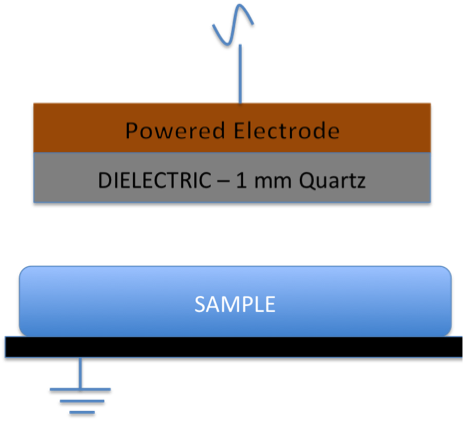
\includegraphics[width=0.5\textwidth]{Figures/DBD}
\caption{DBD}
\label{fig:DBD}
\end{figure}

%DBDs have been shown in laboratory conditions to be effective for bacterial killing \cite{Daeschlein2012in, Fridman2006blood}.
%An air DBD, PlasmaDerm has been tested on chronic ulcers in a clinical trial, though the results are not overly promising \cite{Brehmer2015alleviation}, as plasma induced killing of wound colonising bacteria was not long lasting and there did not appear to be any acceleration in wound healing in the plasma treated group compared to the controls.
%The device operates at AC voltage pulses with amplitudes $>$10 kV and a power density of 120 mW/cm\textsuperscript{2} \cite{Brehmer2015alleviation}.



%\cite{Fridman2007comparison} looks at direct and indirect plasma treatment. Using DBD with and without mesh/airflow to try and separate out the roles of ions and reactive species.
%Both use atmospheric air as the gas.
%Both operate at 35 kV, 12 kHz frequency and power density of 0.8 W/cm\textsuperscript{3}.

In terms of operation, there was a study investigating pulsing of DBD, using both micro- and nanosecond pulses, in particular, investigating the homogeneity of the plasma produced. 
It was found that nanosecond pulsing gave a more homogenous plasma, that would ignite more uniformly over a non-uniform surface.
Specifically, patterned (i.e. not flat) agar was used as the target and it was seen that with microsecond pulses, the plasma was more filamentary and some areas didn't ignite at all \cite{Ayan2009application}. 
However, using the nanosecond pulses, the plasma was more uniform over the entire surface.
This is preferable when considering wound treatments, as the wound bed is not smooth.
Further to this, nanosecond pulsed DBD was found to be more effective for bacterial killing \cite{Ayan2008nanosecond}.

%
%\subsubsection{Floating-Electrode Dielectric Barrier Discharge}
%Similar to DBD, the FE-DBD can be used whereby one of the electrodes can be replaced with anything with a sufficiently high charge storage capacity, a so-called, floating electrode (FE). 
%Biological samples and skin are able to do this due to their high water content {\cite{Fridman2006blood}}.
%Good diagrams of the electrodes are shown in {\cite{Fridman2006blood}}.
%Has been shown that FE-DBD can accelerate the coagulation process in the blood. It seems to catalyse the physiological process of clotting rather than exerting a physical influence.


\scriptsize
\bibliographystyle{ieeetr}
\bibliography{/Users/hld523/Bibliography/MyPapers}
\end{document}  